\section{Antecedentes y Estado del Arte}

\subsection{Evolución de NTN en 3GPP}

Resulta revelador observar cómo la estandarización de las Redes No Terrestres ha pasado de ser una mera exploración a convertirse en un pilar fundamental de la hoja de ruta hacia 6G. Aunque los primeros estudios en 3GPP datan de Release 15, fue en Release 17 donde se materializó el soporte normativo para NTN tanto en NR como en tecnologías IoT. 

Uno de los hitos más significativos radica en la incorporación nativa de acceso satelital para NB-IoT y eMTC, junto con adaptaciones críticas como la pre-compensación de Doppler y timing advance extendido. Nguyen et al. \cite{Nguyen2024} ofrecen una visión panorámica de estas tecnologías emergentes, subrayando cómo las constelaciones LEO y GEO, combinadas con payloads transparentes en un primer momento, sientan las bases para una integración más profunda en Releases posteriores. 

Lejos de ser un asunto resuelto, la evolución continúa en Release 18 con mejoras en rendimiento y movilidad, mientras que Release 19 ya explora arquitecturas regenerativas y funcionalidades como Store & Forward para IoT. Particularmente llamativo es el hecho de que estas especificaciones tienden a priorizar la compatibilidad con dispositivos existentes, aunque esto impone ciertas restricciones en eficiencia espectral y latencia variable según la órbita empleada.

\begin{figure}[t]
\centering
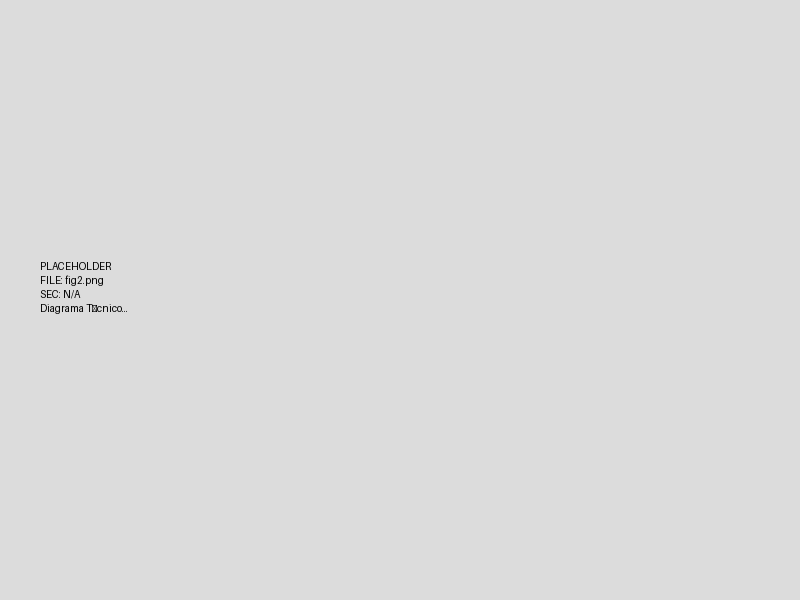
\includegraphics[width=\linewidth]{fig2.png}
\caption{Timeline de la evolución de NTN en 3GPP, destacando Releases 17, 18 y 19 con énfasis en hitos para IoT y multi-conectividad.}
\label{fig:timeline_ntn}
\end{figure}

\begin{table}[t]
\centering
\caption{Comparativa de estándares 3GPP relevantes para NTN-IoT}
\label{tab:comparativa_estandares}
\begin{tabular}{lccc}
\hline
\textbf{Aspecto} & \textbf{Rel-17} & \textbf{Rel-18} & \textbf{Rel-19 (en curso)} \\
\hline
Soporte NTN IoT & NB-IoT/eMTC básico & Mejoras de rendimiento & Store \& Forward, optimizaciones \\
Payload & Principalmente transparente & Transparente + inicial regenerativo & Regenerativo avanzado \\
Handover & Básico & Mejorado & Seamless TN-NTN \\
Eficiencia energética & Limitada & Optimizaciones iniciales & Enfoque prioritario \\
Escenarios & GEO/LEO & + HAPS & Multi-layer integration \\
\hline
\end{tabular}
\end{table}

\subsection{Tecnologías IoT en Entornos Satelitales}

Uno de los desafíos persistentes al integrar IoT con segmentos satelitales consiste en equilibrar la restricción energética de los dispositivos con las demandas impuestas por canales de propagación largos y variables. En muchos casos estudiados, los dispositivos NB-IoT y LTE-M experimentan un aumento notable en consumo durante uplinks hacia satélites, especialmente en constelaciones LEO donde el Doppler y los handovers frecuentes exigen mayor procesamiento. 

Plastras y colaboradores \cite{Plastras2024} realizan un análisis profundo de estas dinámicas energéticas en IoRT (Internet of Remote Things), destacando que, si bien NTN extiende drásticamente la cobertura, no siempre garantiza eficiencia comparable a redes terrestres densas. No obstante, cabe matizar que técnicas como transmisión discontinua, optimización de random access y algoritmos de predicción de visibilidad satelital están cerrando progresivamente esta brecha. 

La literatura reciente parece sugerir que la verdadera ventaja radica en escenarios remotos o de respaldo, donde la alternativa terrestre simplemente no existe.

\subsection{Aplicaciones en Smart Cities}

Aunque las Smart Cities se asocian tradicionalmente con despliegues terrestres ultra-densos, la realidad muestra que muchas aplicaciones críticas —monitoreo ambiental en periferias, gestión de flotas en corredores logísticos o resiliencia ante desastres— demandan conectividad que trascienda los límites de las torres convencionales. 

Aquí es donde las arquitecturas híbridas TN-NTN cobran especial relevancia. Shang et al. \cite{Shang2024} demuestran mediante análisis de multi-conectividad MIMO cómo combinar enlaces terrestres y satelitales mejora sustancialmente la probabilidad de cobertura y la tasa de datos alcanzable, especialmente en entornos urbanos con obstrucciones variables. 

Plastras2024 complementa esta visión al enfatizar el rol de NTN en aplicaciones de monitoreo remoto dentro de ecosistemas urbanos extendidos, aunque identifica brechas energéticas y de latencia que aún requieren atención. Resulta particularmente interesante cómo estas soluciones híbridas no reemplazan a las redes terrestres, sino que las complementan de forma inteligente, creando un continuum de conectividad que parece esencial para las ciudades verdaderamente inteligentes y resilientes del futuro próximo.